\documentclass[11pt]{article}
%%%%%%%%%%%%%%%%%%%%% Load math packages and options
\usepackage{amsmath}
\usepackage{amsfonts}
\usepackage{amsthm}
\usepackage{mathrsfs}
\usepackage{enumerate}
\usepackage[dvipsnames]{xcolor}
\usepackage[T1]{fontenc}
%\usepackage[framed]{listings}   % for code listings other than matlab
\usepackage[framed,numbered]{matlab-prettifier}
% turn "backspace" character (ASCII 8) into a tab (9) to avoid Matlab warning backspace
\catcode8=9
\lstset{
  style             = Matlab-editor,
  basicstyle        = {\ttfamily\tiny},
  mlshowsectionrules = true,
  upquote           = true
}
%  basicstyle        = {\def\fvm@Scale{.80}\fontfamily{fvm}\selectfont\color{Maroon}},
\newcommand\ph\mlplaceholder

\usepackage{graphicx}
%\usepackage{hyperref}  % for adding web-links to pdf documents
\usepackage{verbatim}

%%%%%%%%%%%%%%%%%%% Set margins and basic spacing
\textwidth=6.6in
\textheight=9.8in
\oddsidemargin -0.3in % left margin relative to "standard"
\topmargin -0.7in
\parindent 0in   % paragraph indent
\parskip 0.3cm   % space between paragraphs

%%%%%%%%%%%%%%%%%%  Define some useful shortcuts for parentheses that scale
\newcommand{\p}[1]{\left( {#1} \right)}
\newcommand{\s}[1]{\left[ {#1} \right]}

%\renewcommand{\baselinestretch}{1.1}    % for double spacing use 2.0 (or 1.5)
%%%%%%%%%%%%%%%%%%%%%%%%%%%%%%%%%%%%%%%%%%%%%%%%%%%%%%%%%%%%%%%%%%%%%%%%%%%%%%%%%
%%%%%%%%%%%%%%%%    BEGIN DOCUMENT
%%%%%%%%%%%%%%%%%%%%%%%%%%%%%%%%%%%%%%%%%%%%%%%%%%%%%%%%%%%%%%%%%%%%%%%%%%%%%%%%%
\begin{document}
\pagestyle{empty}    % style "plain" gives page numbers at the bottom

\centerline{\bf Glacier Retreat and Vegetation Change: A Spatial Analysis}
\normalsize
\centerline{\bf Sahil Lalwani }      

\begin{comment}
\subsection*{Typesetting matrices}
Matrices can be tricky to format correctly.
The {\em amsmath package} provides many matrix functions.
For square brackets use the \lstinline|bmatrix| environment.
$$
{\bf A} = \begin{bmatrix}
2 & 4 & -6 \\
1 & 5 & 3 \\
1 & 3 & 2
\end{bmatrix}
$$

% Blank lines denote a new paragraph.

\subsection*{Subsections}
Use \lstinline|\subsection| (or \lstinline|\subsubsection|) for each problem.
\end{comment}

\section*{Introduction to the problem: glacial retreat and vegetation change}

As air temperatures rising under global cliamte change, areas covered in snow and ice are melting. Glaciers are masses of ice that are currently melting as air temperatures increase. Glaciers form when more snow accumulates than melts or evaporates and the snow becomes compacted over time. Glaciers are defined as being persistent over time (don’t disappear seasonally or even every few years) and must be at leat 0.1 km squared in area, and often take thousands of years to form. Glaciers often form in mountainous regions. Glacier National Park is located in Montana and known for sweeping views of glacier covered mountains. The glaciers in Glacier National Park formed at least 7,000 years ago. However, the glaciers in Glacier National Park began noticibly shrinking over the last century. There is concern about impacts on tourism, ecosystems, and hydrology as the glaciers disappear. As shown below, the receding glaciers are changing the landscape.

\begin{center}
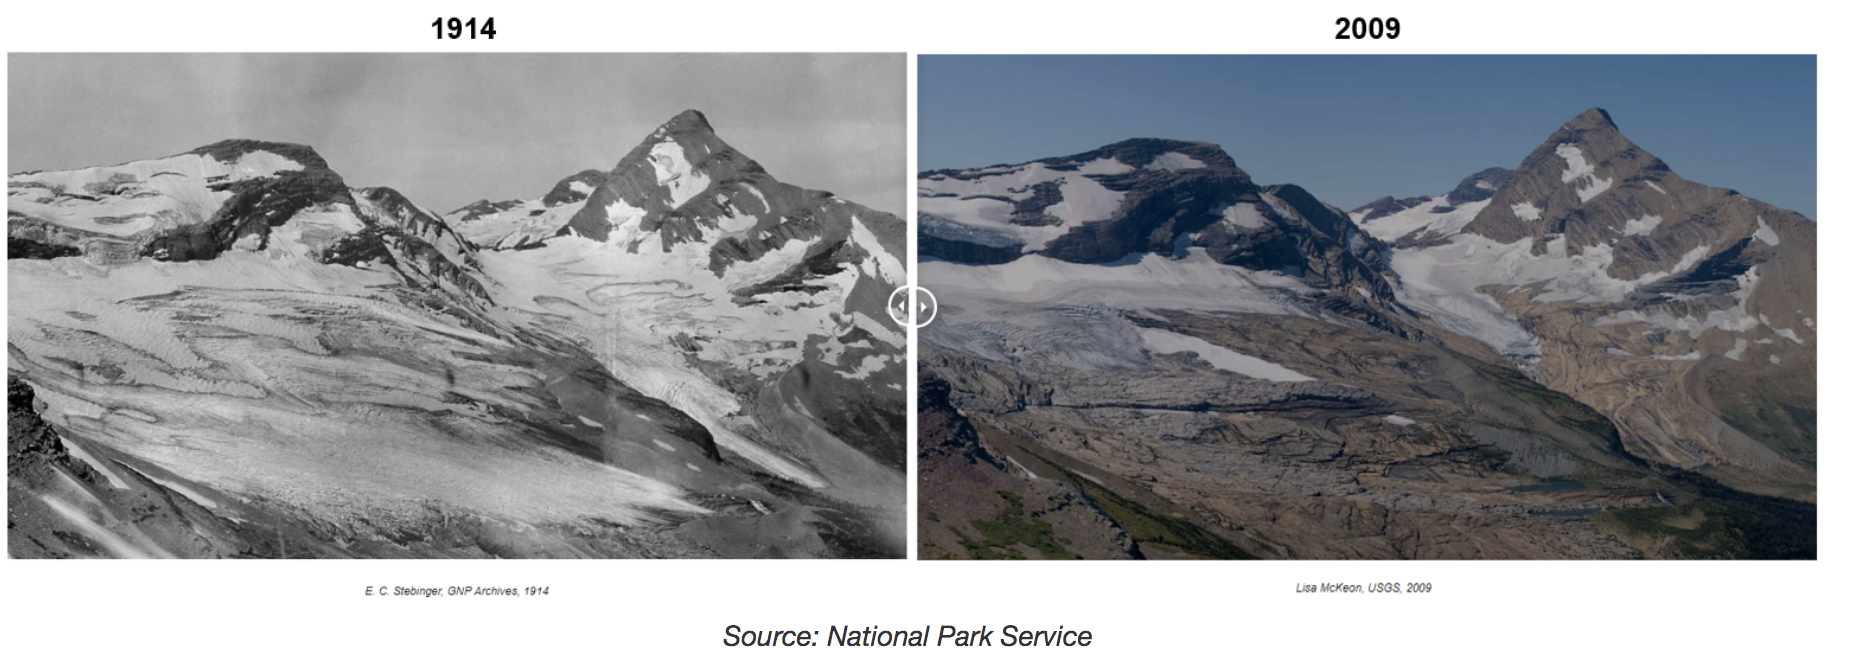
\includegraphics[width=6in, height= 3in]{glacier_retreat_intro.png}
\end{center}

Glacial retreat will drastically affect the regional hydrology, vegetation, and the energy balance. For example, a surface with snow or a glacier reflects more incoming solar radiation off of the earth’s surface compared to bare rock and vegetation nearby. The loss of glaciers means that the land surface will experience even greater warming as more solar energy is absorbed. As glaciers retreat and overall snow and ice cover decreases in mountainous regions, vegetation can grow in newly formed bare surfaces. As seen in the picture above, there is grass growing in areas that were once covered in snow and ice. This growth of vegetation can drive additional change on the land surface and alter water, energy, and carbon cycling. A study by Carlson et. al. in 2017 demonstrated that less snow cover during the year drives increased vegetation in the French Alps. Another recent study by Karen Anderson et. al. in 2019 found that the Himalyas are experiencing increased vegetation growth as glaciers and permanant snow cover retreats.\\

Here, we use data from the National Park Service that shows the footprint of 39 glaciers in 1966, 1998, 2005, and 2015 to show the change in glacier extent over recent decades. We’ll also look at a satellite derived measure of vegetation called the Normalized Difference Vegetation Index (NDVI). NDVI Values ranging from 0 to 1 indicate the relative amount of photosynthetic material on the ground. Values close to one indicate a higher level of vegetation and zero indicates no vegetation. The overall value will depend on characteristics of vegetation, and areas completely covered in vegetation do not necessarily correspond to an NDVI value of one. NDVI varies seasonally and typically peaks in the summer for many cold winter ecosystems. The maximum NDVI value indicates the highest amount of vegetation that year. Tracking changes in NDVI throughout time can indicate if there is increasing or decreasing amounts of vegetation.\\

\subsection*{Reading in Vector Data}

We start by reading in the vector data of the glacier outlines. These glaciers have been digitized by the National Park Service. In shapefiles, all metadata is contained in the .xml file. The GNP\_glaciers file contains all four shapefiles for each year.\\

Note that there are 39 features (glaciers) for each shapefile and a table with information about each glacier that has 13 columns of data.\\

Below, we make a map of the glaciers and view them by name.The spplot function allows you to map vector data and show different colors for a data value. Let’s look at the 1966 glaciers by glacier name.\\

\begin{center}
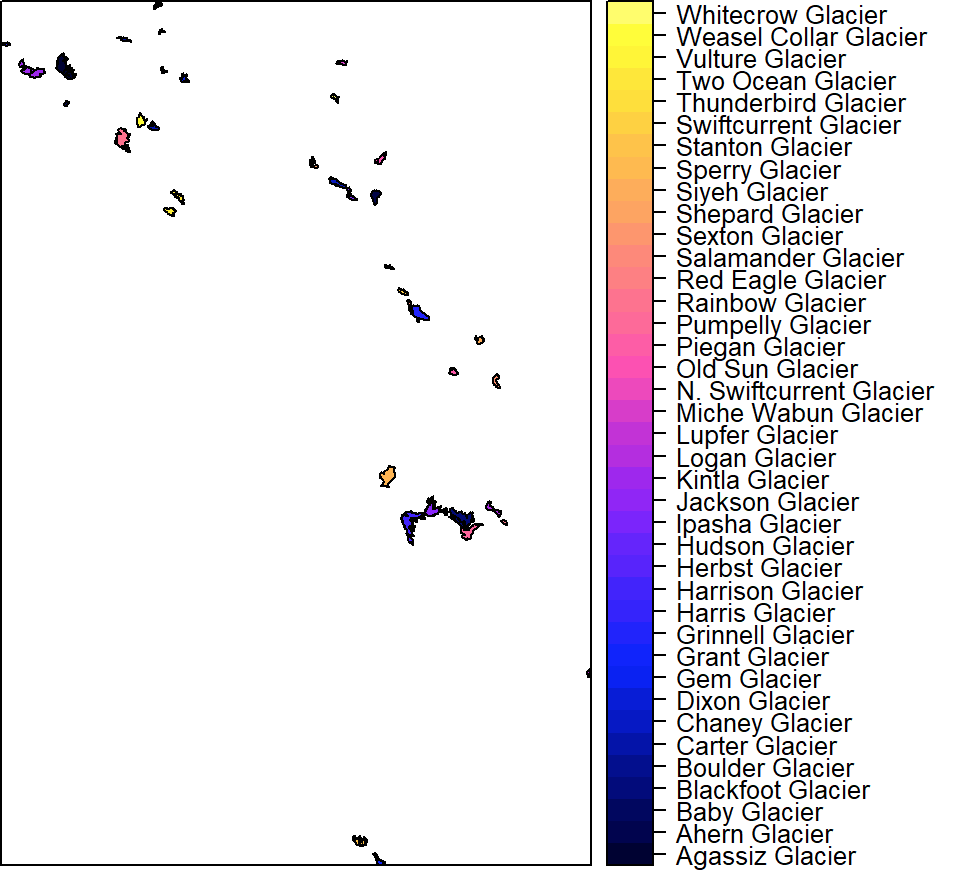
\includegraphics[width=6in]{glacier_by_name.png}
\end{center}

\subsection*{A brief description of the Projection and Datum}

Datum is a model of the shape of the Earth. We generally use a reference datum to record a location in a coordinate pair. In addition, datum also describes or references the longitude and latitude grid that covers this shape of the Earth. In other words, a datum describes the surface of the Earth and the position of the surface relative to the center of the Earth. A
datum may also be understood as a reference point, surface or axis on an object against which measurements are made.\\

Here, the value assigned to datum for g1966 vector data is NAD83. NAD83 provides latitude
and longitude and some height information using the reference ellipsoid GRS80, and is a unified
horizontal or geometric datum that provides a spatial reference for Canada and the United
States.\\

A projection is a series of transformations which convert the locations of points on a curved
surface (the datum which acts as a reference surface) to locations on a flat plane. Simply put,
the projection allows us to locate points on the curved surface of the Earth on a 2-dimensional
plane or surface. It is important to note that datum is integral to the interpretation of the
projection. The same point projected in XY-coordinate system may have different latitude/
longitude values under different reference datum.\\

Here, the projected coordinate system is UTM (Universal Transverse Mercator) which is also
one of the most common mercator projection systems. The UTM system divides the Earth into
60 zones, each 6° of longitude in width. In UTM system, the center is along lines of longitude.
The highest area of accuracy is in the center of each zone. As a result, the system maintains a
more realistic representation of distance, area and shape within each zone compared to other
projection systems. In fact, there is almost no distortion in the projection along the line of
longitude. The narrow width of each zone and limited distortion between lines of latitude in the
UTM system exist because we move only a small distance laterally.\\

Within the UTM projection system, any coordinates have to be referenced to the central
meridian of a given UTM zone. Coordinates are given in meters and not degrees. In order to
better understand zones, it is important to understand that the UTM projection system uniquely
allows us to project each of the 60 zones onto a plane separately rather than projecting the
complete globe onto a flat surface. Here, the UTM zone is 12 which has a central meridian at 111° W and its extent us 114°W-108°W. In order to better contextualize these results, we note
that each UTM grid cell has a central meridian of 500,000m.\\

In light of the above, it is clear that the UTM projected coordinate system is meant for particular
areas (smaller zones) rather than a global spatial scale. Thus, the spatial scale of this projected
coordinate system is restricted to relatively narrow strips of land compared to the area of the
whole globe.\\

\subsection*{Data Cleaning}

Before we get started with analysis, there’s one other issue. The glacier names in 2015 don’t match the rest of the shapefiles. We notice Miche Wabun is missing Glacier in its name and North Swiftcurrent Glacier should be abbreviated as N. We fix that so you can use the glacier names as an indexing variable across years.\\

\section*{Working with Raster data}

\subsection*{Mapping satellite imagery}

\textbf{Glacier data}

\begin{center}
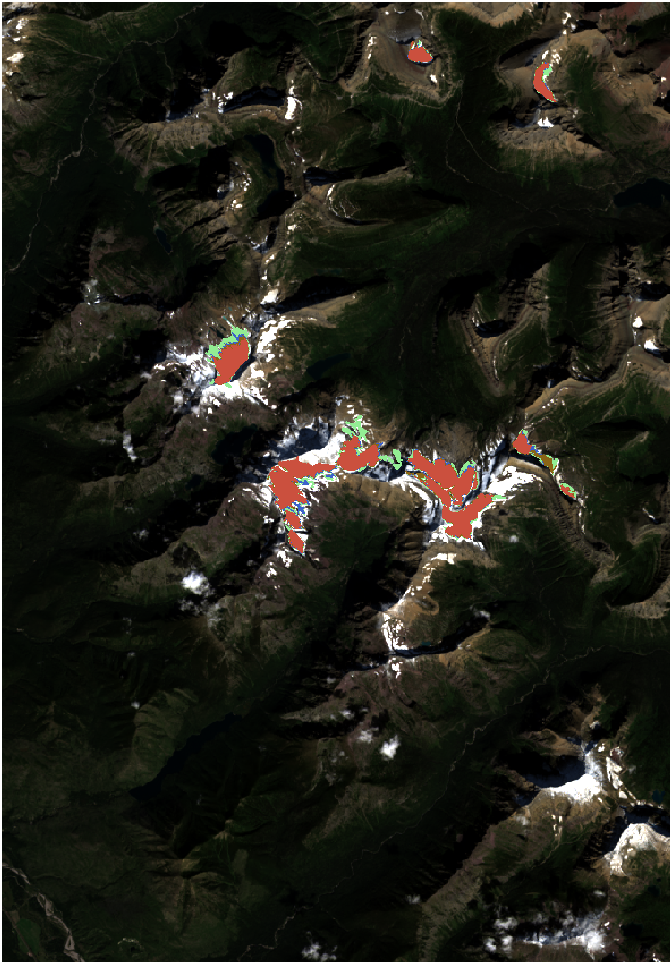
\includegraphics[width=3in, height=3in]{glacier_data.png}
\end{center}

\textbf{NDVI data}

\begin{center}
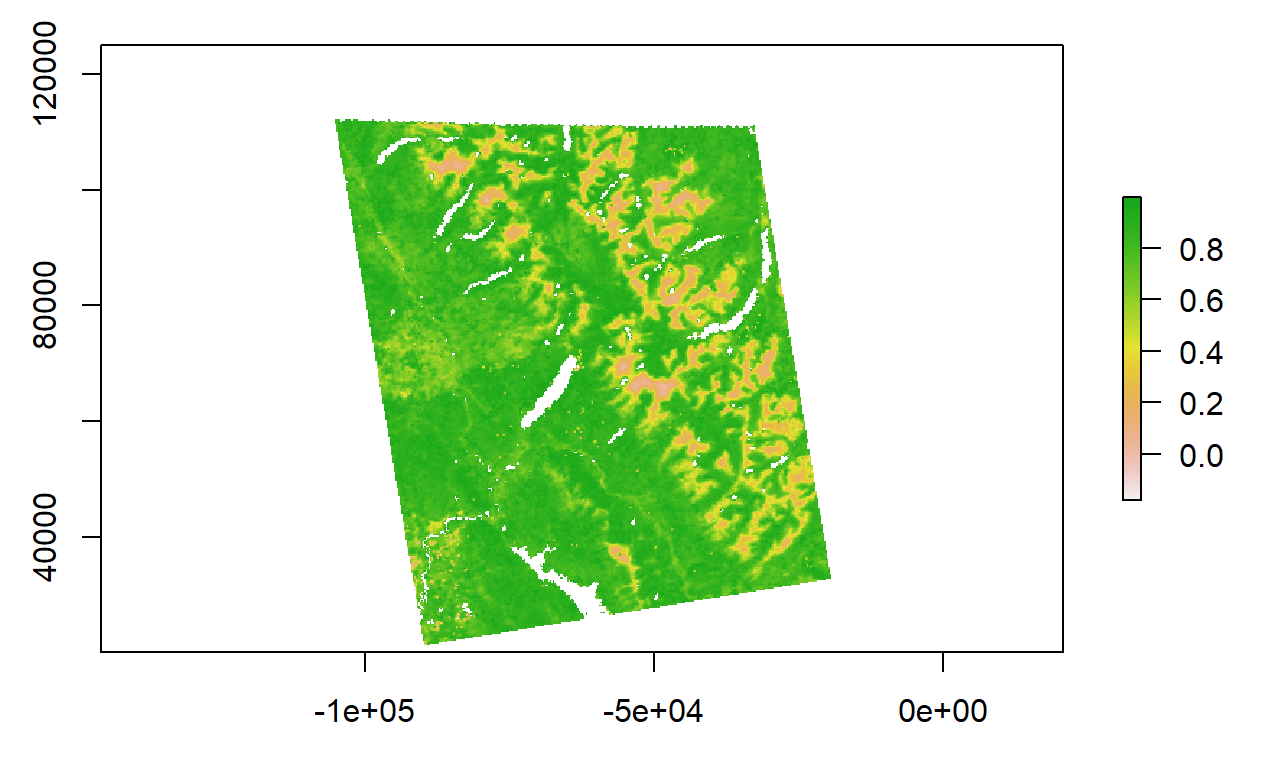
\includegraphics[width=4.8in, height=4in]{ndvi_raster.png}
\end{center}

\section*{Vector Data Analysis: glacier retreat}

Below, we make a map with both the maximum NDVI and the glaciers in 2015.

\begin{center}
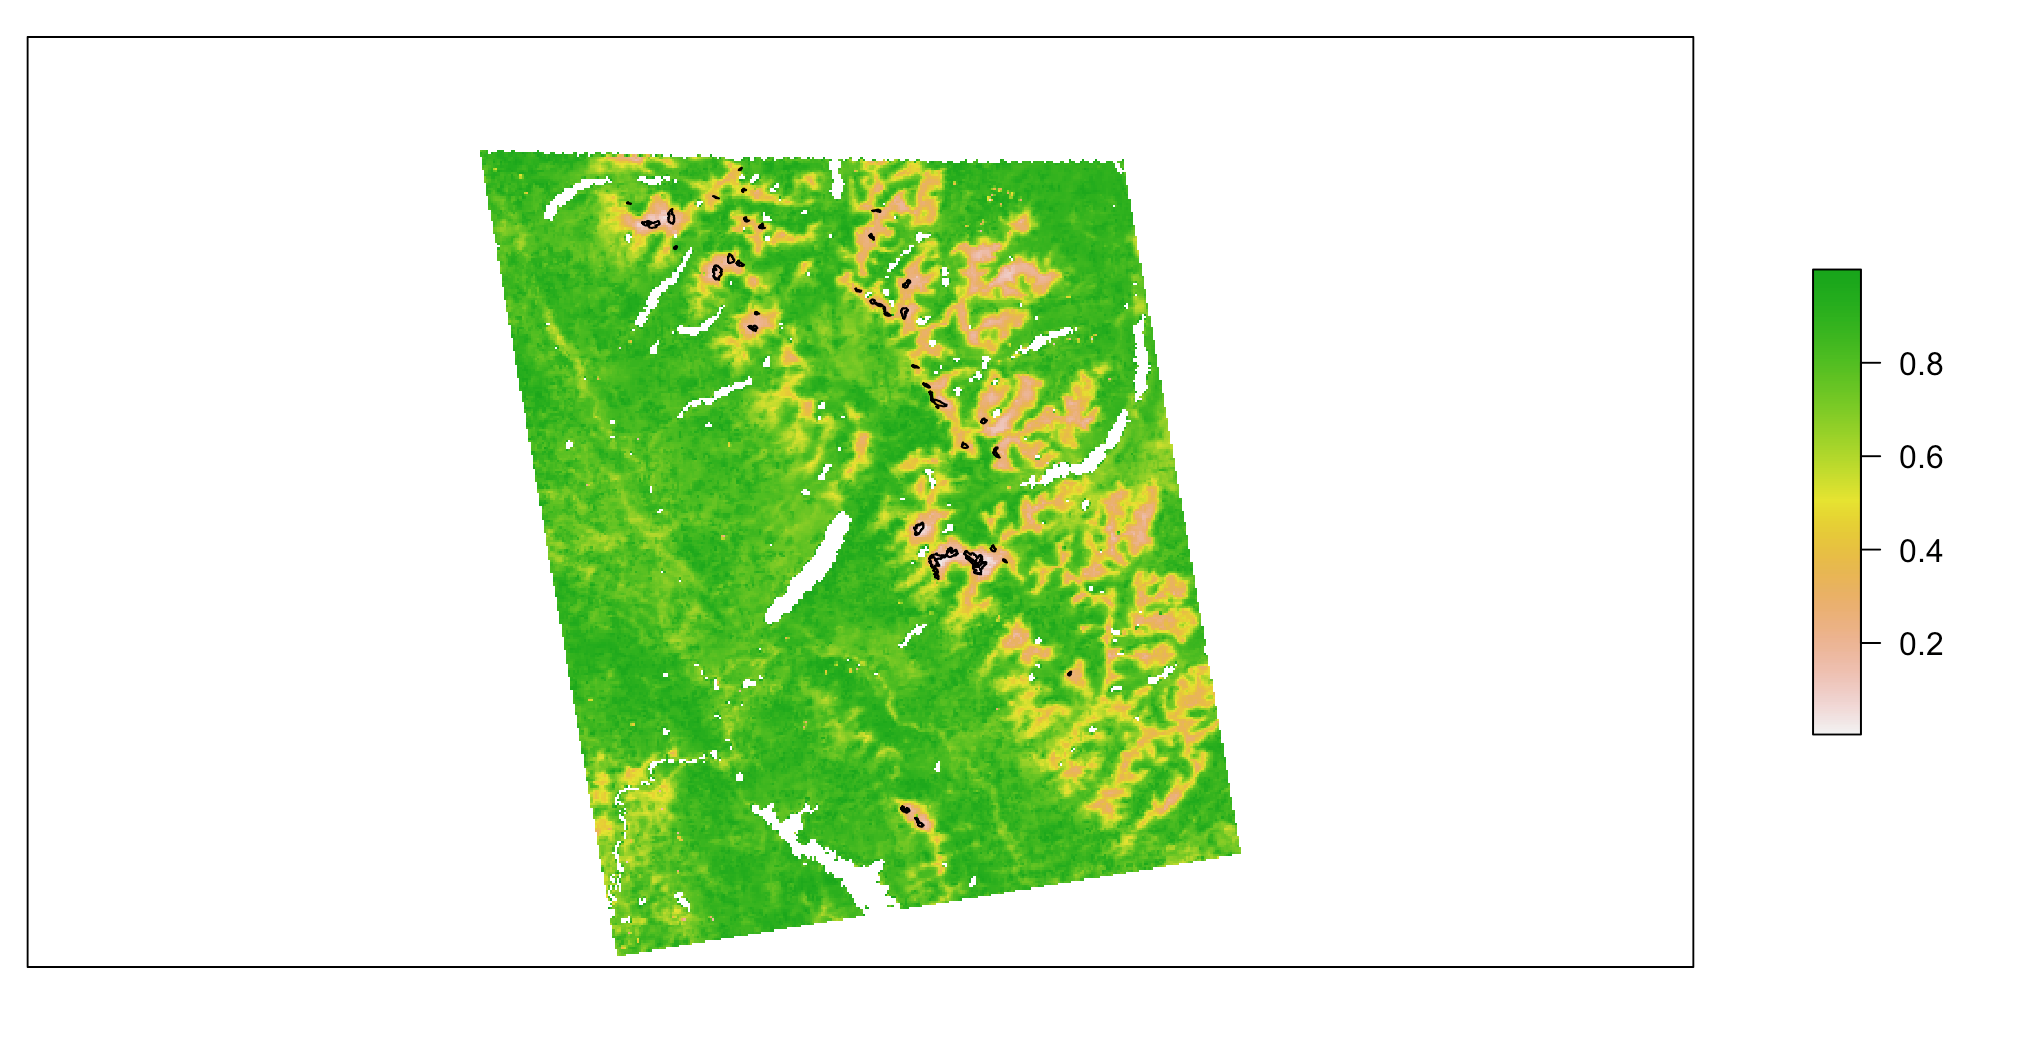
\includegraphics[width=5.2in, height=4in]{q4_new.png}
\end{center}

A few interesting patterns emerge. Overall, a majority of area in the map show high maximum NDVI values close to 1. Thus, a
majority of area in the map has relatively high amount of photosynthetic material on the ground.In comparison, overall, the NDVI values around the glacier are very low (roughly between 0.1
and 0.3) compared to the NDVI values seen throughout the map. We now wish to investigate if
there are any patterns in NDVI values around glacier by two major properties of glaciers:
relative glacier geographical position and glacier size.\\

We note that the area surrounding most glaciers have low NDVI values. This is because
glaciers have a very specific definition- they are persistent over time and must be at least 0.1km
squared in area. However, areas around glaciers are also often covered by snow which implies
a lower relative amount of photosynthetic material in these areas and hence, lower NDVI
values. The areas surrounding glaciers may also be mountains which again have relatively low
NDVI values. It is interesting to note, however, that the areas of land around glaciers having low
NDVI values vary in magnitude.\\

We may suspect that glacier size may potentially affect the area of land around glaciers having
low NDVI values. However, the visualization doesn’t support this claim. We note that some
small glaciers and other large glaciers often have comparable areas around them having low
NDVI values. Thus, we do not see a consistent relationship of NDVI values of areas around
glaciers and glacier size in a direct or inverse manner.\\

We note that geographic position and surrounding characteristics of land uniquely determine the
extent of area of land around glaciers having low NDVI values. Along those lines, we also note
that huge areas of land throughout the map encompassing no glaciers also have relatively very
low NDVI values because they may be mountains or covered in snow but do not meet the
technical requirements to be categorised as a glacier.\\

We must also note that NDVI index is overall a very broad metric to measure the amount of
vegetation in an area. For example, the grass growing on previously snow-covered mountains
we saw in the satellite image is a very small increase in NDVI value around glaciers that is not
effectively captured or visualized in the NDVI map above.\\

\subsection*{Area of glaciers over the years}

\begin{center}
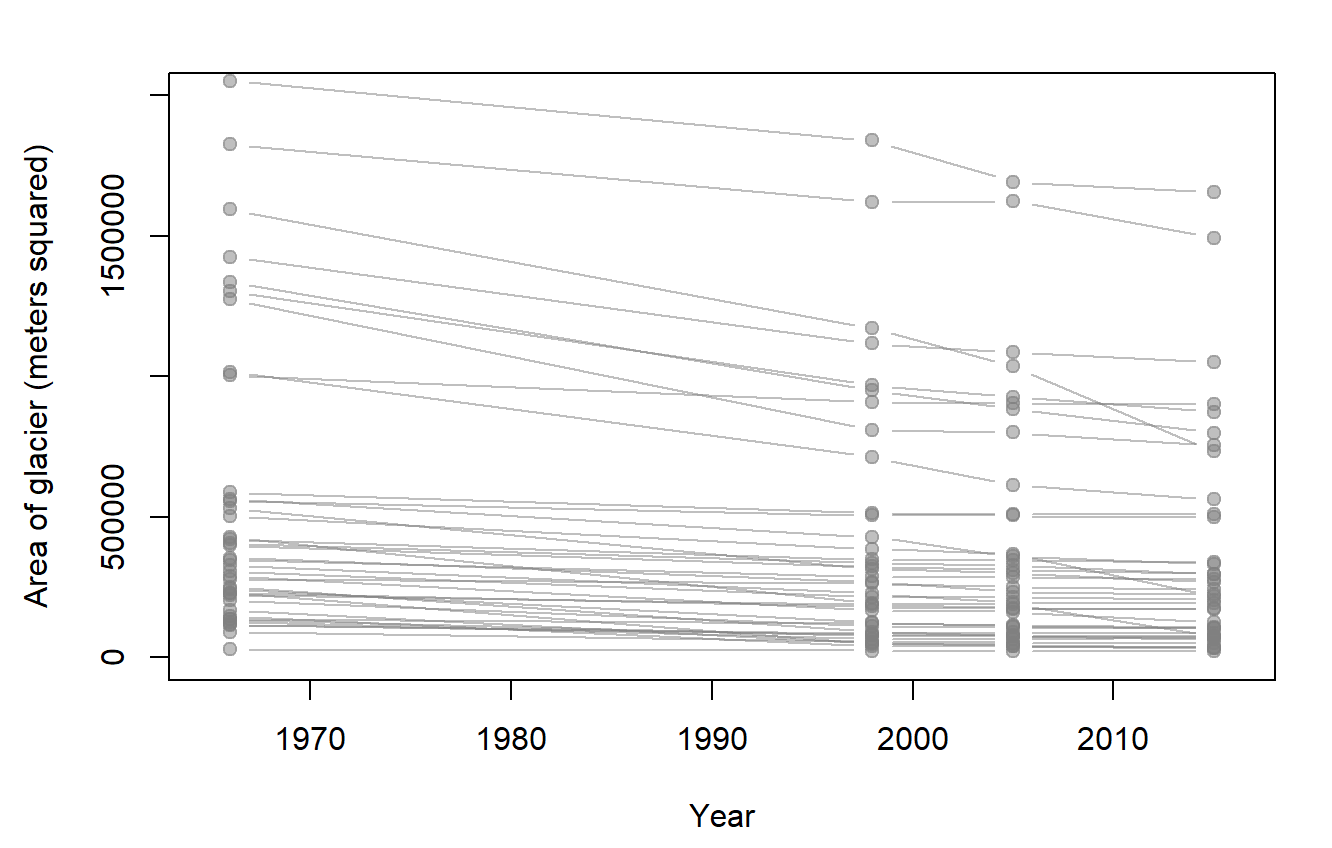
\includegraphics[height=4in]{area_glacier_time.png}
\end{center}

This is a good first look, but it would be more helpful to look at the percent change since small glaciers overall have less area to lose. Below, we make a plot of the glaciers in 2015 showing the percentage change that each glacier has experienced.\\

\begin{center}
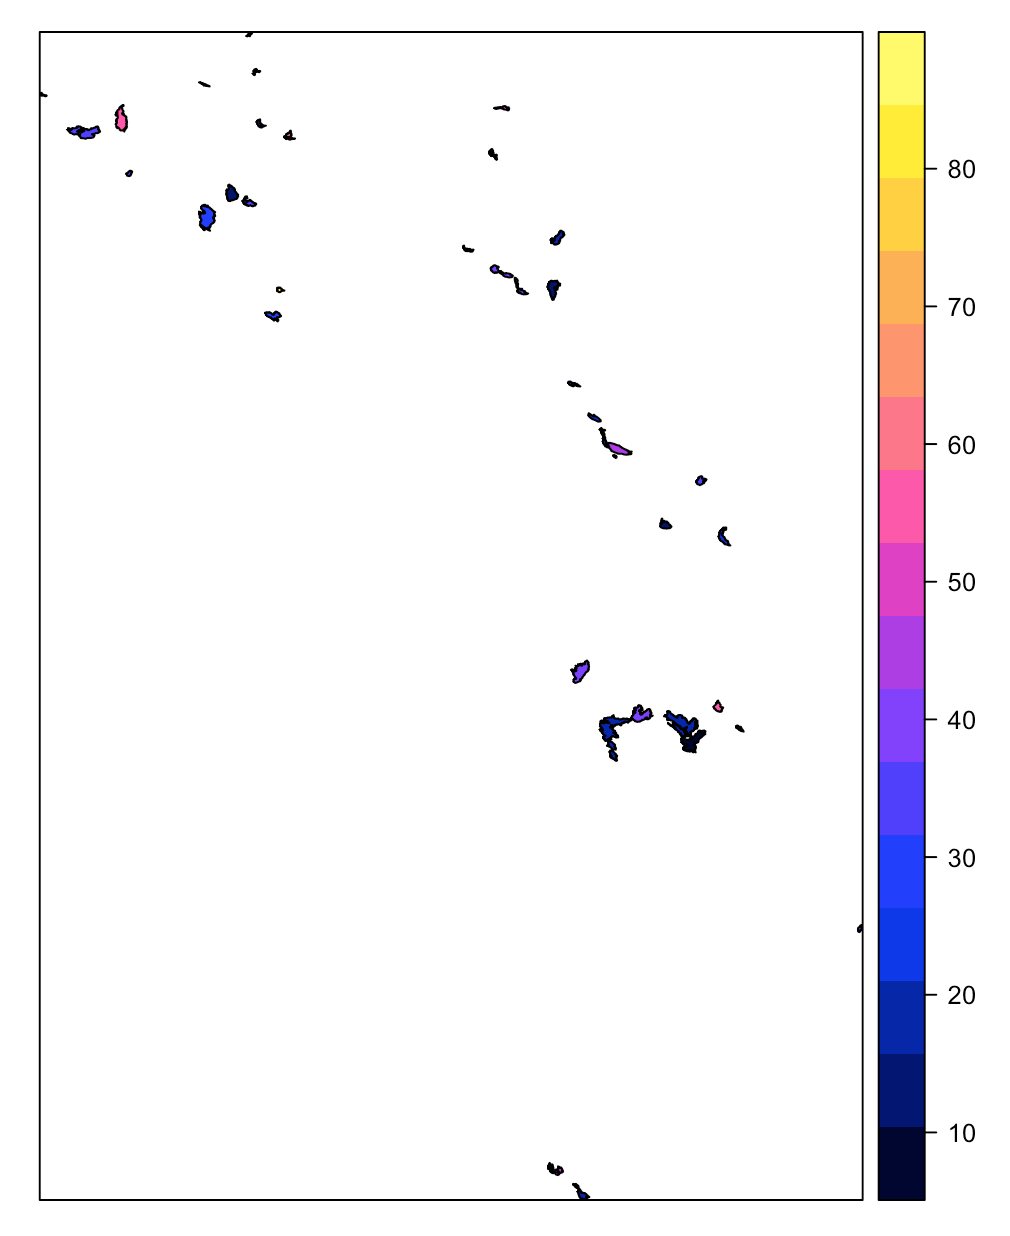
\includegraphics[height=4in]{q5.png}
\end{center}

It might help to visualize the glacial loss more directly. Let’s make a polygon that shows the difference in glaciers between 2015 and 1966.

\begin{center}
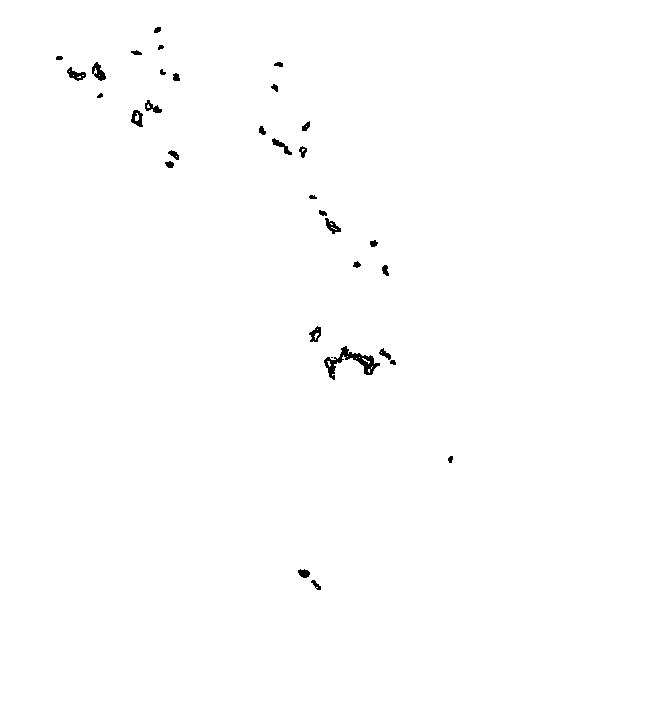
\includegraphics[height=3in]{q5_cont.png}
\end{center}

Below, we create a map that best displays the glacial extent for all years for that glacier with the highest percentage loss.

\begin{center}
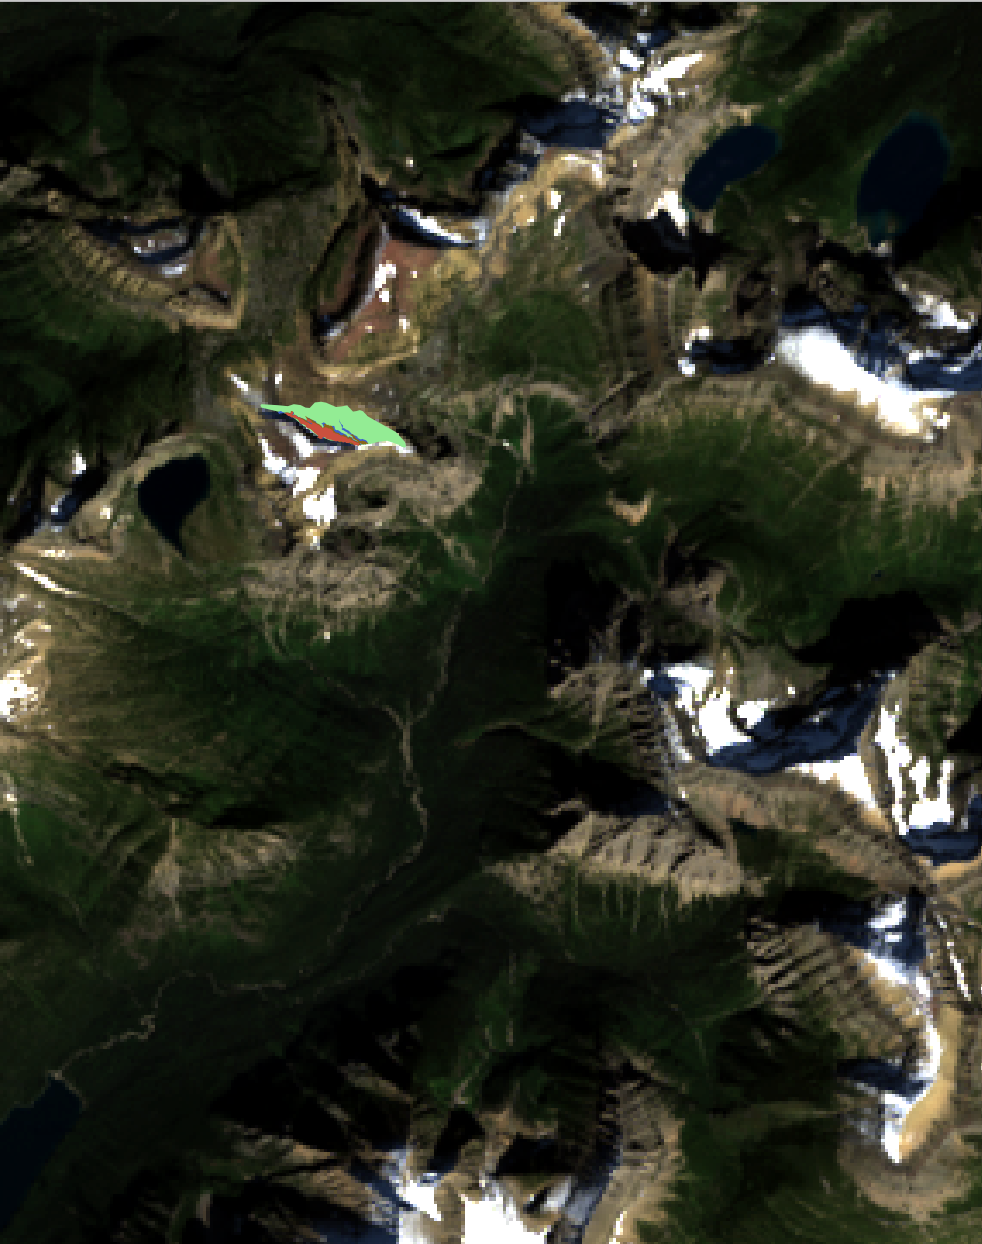
\includegraphics[height=3in]{q6_alt2.png}
\end{center}

The glacier with the largest \% loss is “Boulder Glacier”.

\section*{Raster data analysis: does more vegetation grow with glacial retreat?}

Let’s take a look at patterns in maximum NDVI from 2003-2016 to see if there is an increase in vegetation throughout the time period. Let’s start by examining how NDVI might be changing within the area that glaciers are retreating. We can get all of the values that are within a polygon using the extract function. Let’s extract each year’s NDVI in the area that experienced retreat from 1966 to 2015 and take the average.\\

Although 2015 had very high NDVI, it doesn’t appear that there is much of a trend.This is not surprising because it may take many years for vegetation to move in and fill in a newly bare glacial area. There may also be prolonged snow cover in many of these areas even if there is not a glacier there. \\

\begin{center}
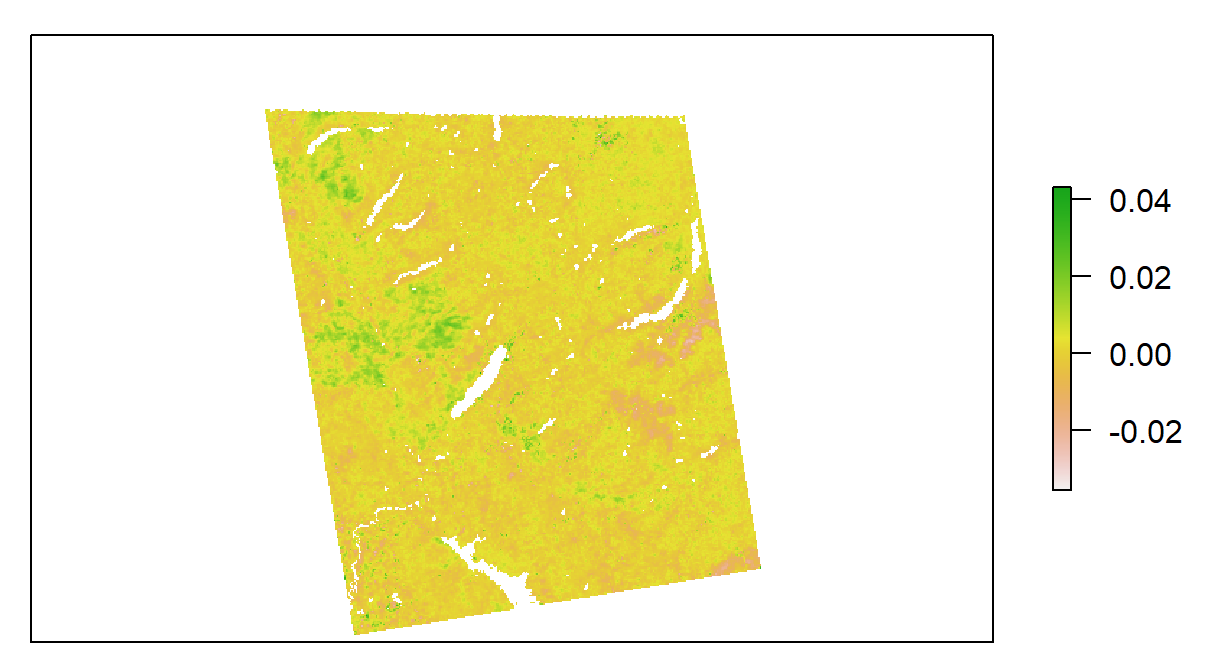
\includegraphics[height=3in]{q7.png}
\end{center}

\subsection*{Discussion of patterns in maximum NDVI change across the park}

Visually, it seems that a majority of area within the map has experienced minimal to no change
in the maximum NDVI value. We also note some areas of land within the map which are not
colored and represent areas which are not eligible to be assessed in terms of NDVI changes.
Such areas may include bodies of water. We do note that a relatively higher maximum NDVI
change is concentrated in areas of land geographically close to one another. We may suspect
such areas experiencing high NDVI value change per year to be areas at low elevation. It is also
clear that a large amount of area in this map representing mountains and areas covered in snow
(but which are not glaciers) experience very little, if any, NDVI change per year.\\

We can see light green colored areas of land near some glaciers suggesting an increase in the
relative amount of photosynthetic material (or vegetation) in areas of land surrounding glaciers.
However, this analysis is limiting for a major reason. The NDVI increase in areas surrounding
glaciers may be so small (like the growing of grass in previously snow covered mountains) that it
may not be visible in the broadly defined scale for the color spectrum in the above plot. Thus,
we need to focus our analysis specifically on studying NDVI changes across areas surrounding
glaciers\\

However, we note that we haven’t checked if the value of the slope for the change in NDVI per year is statistically
significant. In other words, we need information on the p-value of the slope to check if the value
of the slope is significantly different from 0. This is particularly important considering the value of
the slope is expected to be very small (close to 0) for areas surrounding the glaciers because
the increase in vegetation in these areas, if any, will not be as high as those in low elevation
plains or areas of land. This expectation is supported by the data. Thus, we need to know if the
value of the slope is significantly different from 0 to proceed with the analysis and interpret the
results of the analysis correctly.\\

\section*{Results}

Below, we map the mean change in NDVI per year into the 2015 glacier polygons:

\begin{center}
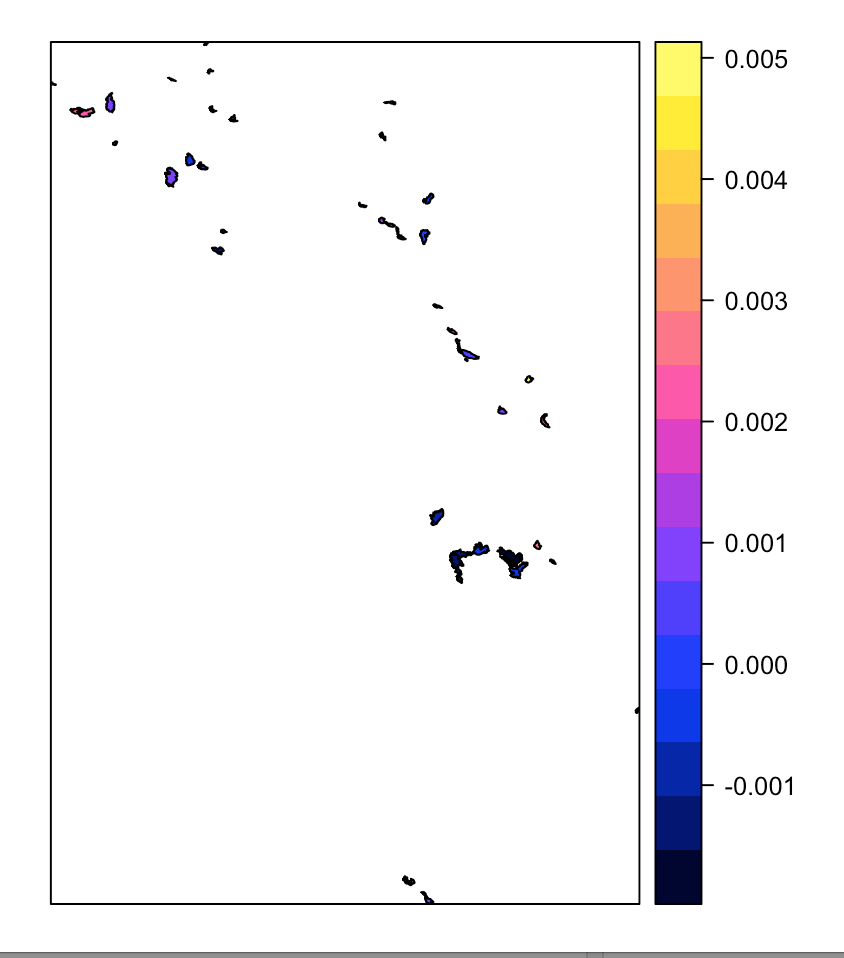
\includegraphics[height=3in]{q9.png}
\end{center}

The mean change in NDVI per year across all glaciers is low in magnitude, ranging
between 0.001 and 0.005. A majority of 2015 glaciers seem to have a mean change in NDVI on
the relatively lower end of the spectrum, meaning between -0.001 and 0.001. A few glaciers are
seen to have mean NDVI change per year greater than or equal to 0.002.\\

No consistent pattern is seen within this map. For example, a few glaciers having relatively high
mean changes in NDVI per year comprise a variety of sizes. I believe that the mean change in
NDVI per year for a glacier is highly dependent on the particular geographic location and
characteristics of a glacier.\\

\textbf{Main takeaway:} I think vegetation is changing as glaciers recede. The range of mean change in
vegetation we obtained in our analysis in the previous question is [-0.0012, 0.004]. The
magnitude of the range seems significant, because a slope value of -0.003 over a 15 year
period would decrease NDVI by 0.045. This may not seem like a significant increase in NDVI
because, as we saw in our map for question 4, most area throughout the map other than that
covered by glaciers, snow or mountainous has very high NDVI values (close to 0.6 or 0.8).
However, this change is important to be considered for a few reasons.\\

Firstly, the increase in NDVI value of areas covered by glaciers or snow will obviously be
relatively far lower in magnitude than the increase in NDVI value of low elevation areas with
high vegetation. For example, the images of the mountains show grass growing on the
mountain area previously covered by snow. Growing of grass doesn’t significantly increase
NDVI values, but significantly alter the ecology of previously glacier covered areas. In fact, both Carlson and Anderson paper also had lower slope values but found a significant change in
vegetation when validated with an analysis of imagery. Secondly, low slope values are not very
well contextualized in our parametric model. When we consider the whole map’s NDVI values, it
seems to be a very left skewed distribution with glacier and its surrounding area’s NDVI values
occupying the left skewed portion of the distribution. Instead, I believe that using a
nonparametric alternative like Mann-Kendall tests will rank the NDVI value and is expected to
show that the change in NDVI values seen is, in fact, related to a significant change in
vegetation in the area. The conclusion, in our case, on whether glaciers receding is related to a
change in the vegetation in the National Park is also dependent on whether the value of the
slope obtained under our parametric regression model is significantly different from 0.\\

Lastly, the value of the slope for 74% of all glaciers is positive. Thus. I believe that a decrease in
glacier extent has been related to a positive increase in vegetation. Of course, as in Carlson’s
paper, negative changes in vegetation may be justified using the existence of certain specific
local factors and geographical location of these glaciers. In Carlson’s paper, he justifies the
negative slope values using local conditions like forest fires, agricultural practices etc. Thus, a
consistent relationship between change in glacier extent and the corresponding direction of
change in vegetation may not be established such that it holds true always.\\

Map that shows both the most recent glacier extent color coded with the surrounding maximum
NDVI average, and use the raster of average maximum NDVI as a basemap :

\begin{center}
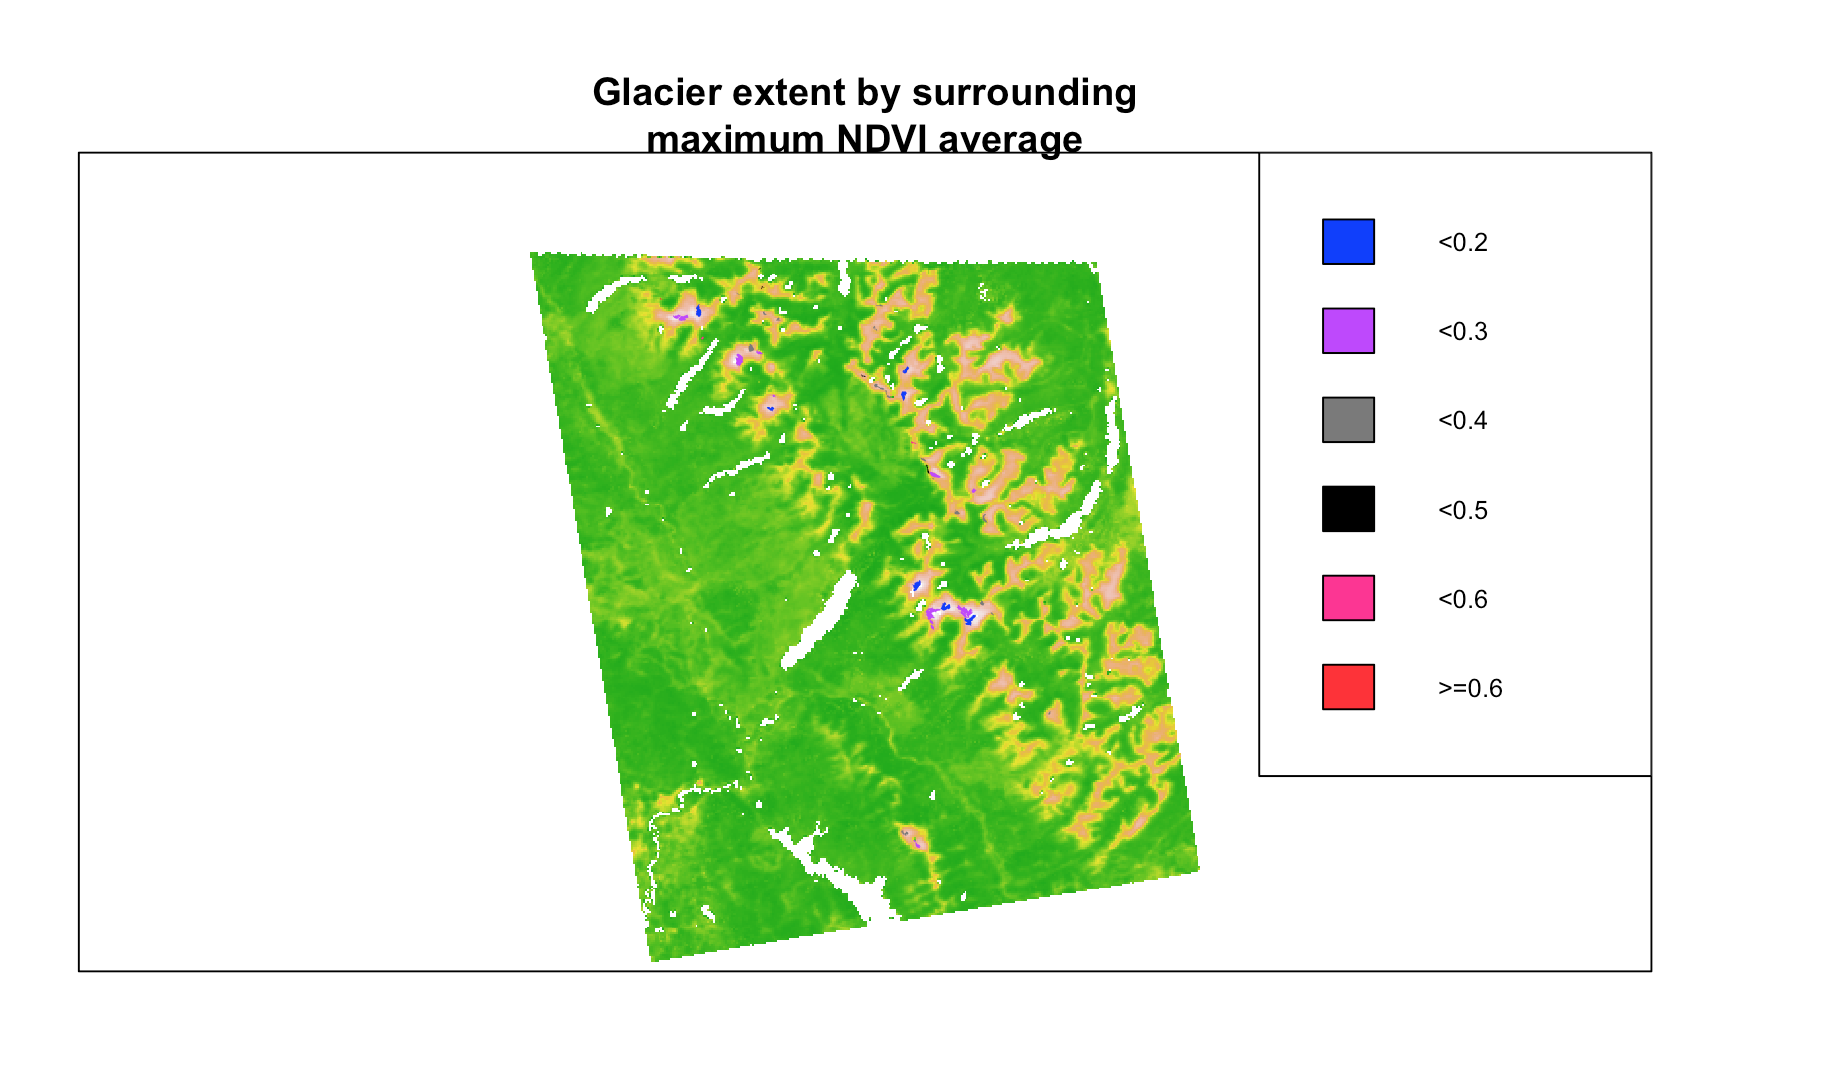
\includegraphics[height=3in]{q11.png}
\end{center}

Using the map below, there doesn’t seem to be a consistent pattern between glacier size and
the average NDVI across all years within 500m. Instinctively, it initially seemed to me that
average NDVI within 500m and glacier size are inversely related, as red areas representing high
average NDVI were relatively small in area while blue and purple color code areas representing
low average NDVI values seemed relatively large in area. However, we also see very small
areas of land colored blue (representing relatively lower average NDVI values) and relatively
large areas of land colored pink (representing relatively higher average NDVI values). Overall, I
have failed to see a consistent pattern of glacier size and average maximum NDVI for all years
for glaciers within 500m.

\begin{center}
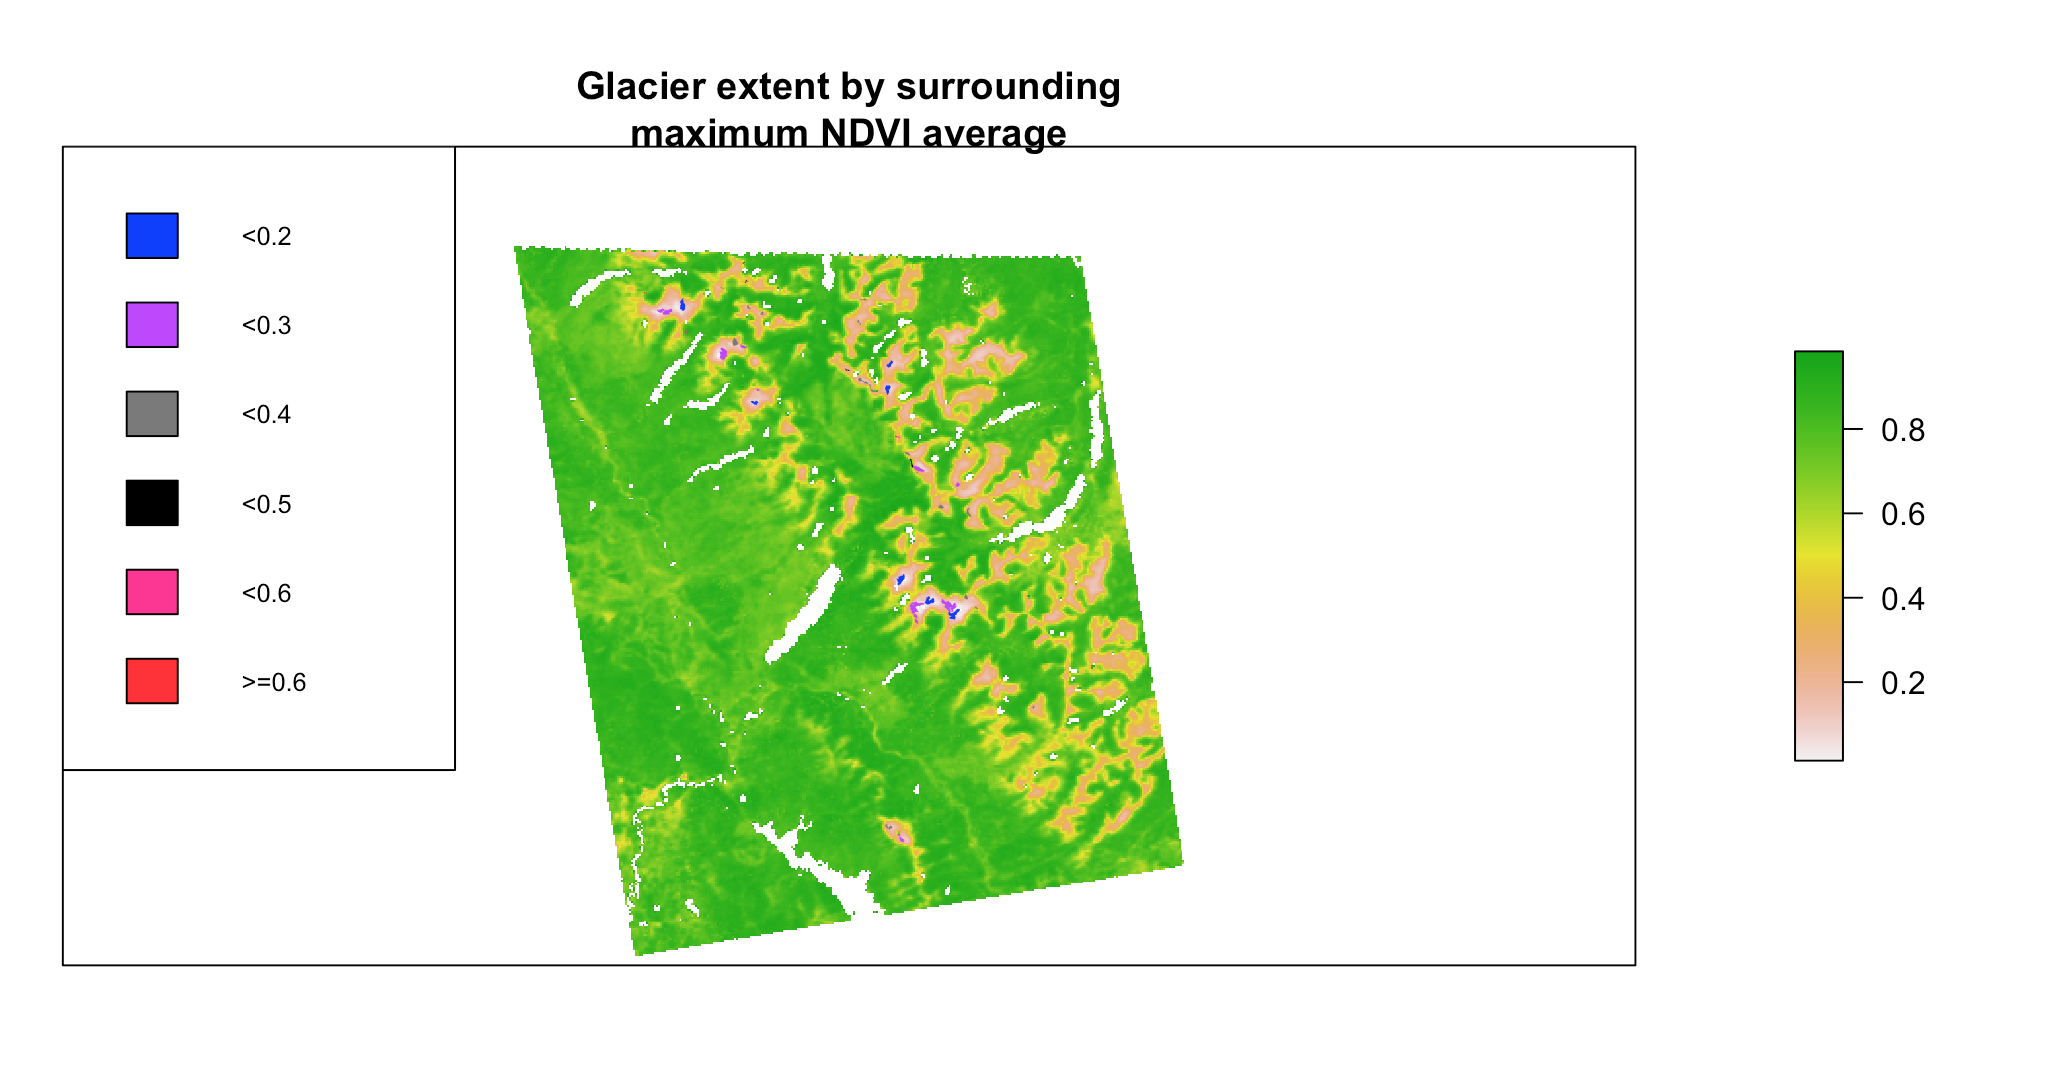
\includegraphics[height=3in]{q11_2.png}
\end{center}

\subsection*{Past Literature and Scope for Further Research}

According to the Anderson paper, we would need online photographs to validate what is
happening with vegetation as glaciers recede. In fact, ecological information is available via
public accessible photographs accessible through Google. In fact, Photosphere
and StreetView images provide a means by which basic ecological data can be gathered (i.e.
presence/absence of vegetation;and broad categorical classifications of the type of vegetation;
e.g. grass/shrub). The results from analysis of satellite data may be compared to the ecological
data conveyed by these photographs. Obtaining this data has not been conventionally easy,
particularly because obtaining such data requires a manual inquiry of photographs to digitize
ecological data. Secondly, Anderson also suggests that we need more ecological studies to
have ecological datasets available for validation.\\

Similarly, Carlson’s paper combined imagery from multiple sources (MODIS, Landsat-5, 7, 8)
with land cover data to test for long-term (1984–2015) greening or browning trends of vegetation
in a temperate alpine area, the Ecrins National Park, in the context of recent climate change and
domestic grazing practices.\\

In order to make a more accurate analysis of vegetation change for research, we may expand
the spatial scale to expand the scope of geographical extent of our research. For example, we may move beyond the Glacier National Park in our study to look at a wider geographical area.
Secondly, we may look at a detailed summary of regression to see if the value of the slope is
significantly different from zero. Thirdly, we may combine our temporal analysis of satellite
imagery here with repeat field surveys of plant diversity and multi-trophic community
composition. Fourthly, increased field work is very necessary to not only validate the results of
our analysis but also to explore possible mechanisms for the results of our statistical analysis.
Additionally, we may quantitatively verify some of our visual findings within this finding. For
example, we have an idea that lower elevation areas have higher NDVI values. We may
numerically verify this using the availability of appropriate data to make a scatterplot of NDVI
against elevation and check the correlation coefficient (ideally Kendall’s Tau and not Pearson’s
correlation coefficient). Furthermore, we should also aim at making a more sophisticated model
for NDVI by identifying the right independent variables including elevation, glacier size etc. by
checking the assumptions for regression and using the necessary regression transformations if
necessary. In fact, we may look at nonparametric alternatives of regression like Mann-Kendall
tests which are based on ranked data and produce relatively uniform or proportional results.
Lastly, we must also look to be skilled in image mapping so that we can use data available in
the form of online photographs to map vegetation and validate our findings.\\


\end{document}
%%%%%%%%%%%%%%%%%%%%%%%%%%%%%%%%%%%%%
%%%%%%%   END DOCUMENT
%%%%%%%%%%%%%%%%%%%%%%%%%%%%%%%%%%%%%

After the end of the document, nothing gets processed, so you can keep
convenient Latex idioms to copy and paste when you need them.

%%%%%%%%%%%%%%%% itemize (bullet lists)
\begin{itemize}
\item
\item[a)]
\end{itemize}

%%%%%%%%%%%%%%%% enumerate (numbered lists)
\begin{enumerate}
\item
\item[a)]
\end{enumerate}

%%%%%%%%%%%%%%%% aligned equations
\begin{align*}
   &  \\
   &
\end{align*}

%%%%%%%%%%%%%%%% figures
\begin{center}
\includegraphics[width=3in]{file}
\end{center}

%%%%%%%%%%%%%%%% move vertically or horizontally
\vspace{.2in}
\hspace{-.8cm} {\bf Page , Exercises:}

%%%%%%%%%%%%%%%% code listings
\lstinputlisting{filename.m}

\lstinline|f=@(x,r) r.*x.*(1-x);|    % this leaves the code in the tex (inline)

\begin{lstlisting}[language=matlab]
f = @(x,r) r*x*(1-x);
x = .33;
for i=1:N
    x=f(x,r);
    xvalues(i)=x;
end
\end{lstlisting}
